%&program=pdflatex

\documentclass[11pt]{article}
\usepackage[latin9]{inputenc}
\usepackage[T1]{fontenc}
\usepackage[english]{babel}
%\usepackage[urw-garamond]{mathdesign}
%\usepackage{palatino}
\usepackage{alltt}
\usepackage{enumitem,textcomp}
\usepackage[raggedright]{sidecap}
\usepackage{multicol,multirow,dcolumn,colortbl}
\usepackage{alltt}
\usepackage{verbatim}
\usepackage{graphicx}
\usepackage{mypdfpages}
\includepdfset{pages=-,link,pagecommand={\thispagestyle{empty}}}
\usepackage[svgnames]{xcolor}
\usepackage{amsmath}%,amssymb}
\usepackage{eurosym}
\usepackage[pdftex]{hyperref}   % doit toujours etre charge en dernier (a part geometry): redefinit certaines commandes
\hypersetup{bookmarks=true,colorlinks=true,linkcolor=black,citecolor=black,urlcolor=blue}
\usepackage[a4paper,scale={0.90,0.90},heightrounded,centering]{geometry}
\pagestyle{plain}

\graphicspath{{./}}
%\input abrev

\parindent=0cm

\setlist[description]{labelindent=.5cm,font=\ttfamily \bfseries}

\newcommand{\inlinemaketitle}{{\let\newpage\relax\maketitle}}

\def\msol{\ensuremath{M_\odot}}
\def\teff{\ensuremath{T_\text{eff}}}
\def\om{\ensuremath{\Omega}}
\def\omcrit{\ensuremath{\om_\text{crit}}}
\def\veq{\ensuremath{V_\text{eq}}}
\def\vcrit{\ensuremath{V_\text{crit}}}
\def\rapv{\ensuremath{V/\vcrit}}
\def\omcrit{\ensuremath{\om_\text{crit}}}
\def\rapom{\ensuremath{\om/\omcrit}}
\def\ddh{\ensuremath{D_\text{h}}}
\def\dshear{\ensuremath{D_\text{shear}}}
\def\el#1#2{\ensuremath{^{#1}\text{#2}}}
\def\he{\el{4}{He}}
\def\carb{\el{12}{C}}
\def\oxy{\el{16}{O}}
\def\itembb{\item[\ \ \ \textbullet]}
\def\itemb{\item[\ \ \ \textopenbullet]}

\newlength{\codeindent}
\setlength\codeindent{.5cm}
\newcommand{\codeline}[1]{\hspace*{\codeindent}\texttt{\detokenize{#1}}\\}
\newcommand{\codelineend}[1]{\hspace*{\codeindent}\texttt{\detokenize{#1}}}

\setcounter{tocdepth}{3}
\title{GENeva Evolution Code (GENEC):\\a quick overview}
\author{Cyril Georgy \& Sylvia Ekstr\"om}
%\date{} % delete this line to display the current date

%%% BEGIN DOCUMENT
\begin{document}

\vspace{-.5cm}

\includegraphics[width=.28\textwidth]{GENEC_logo}
\hfill
\begin{minipage}[b]{.48\textwidth}
\inlinemaketitle
\end{minipage}
\hfill
\begin{minipage}[b]{.2\textwidth}
~~~~~~~~~~~~~~~~~
\end{minipage}
\vspace{.1cm}
\hrule
\tableofcontents
~
\hrule
\newpage
%********************************************************************************************************
\section{Program}
%----------------------------------------------------------------------------------------------------------------------------------
\texttt{GENEC} is the stellar evolution program of the Geneva group. It is composed of a main program and 33 associated modules written in fortran 90.\\

It is maintained on \href{https://github.com/GESEG/GENEC}{GitHub}, in the \href{https://github.com/GESEG}{GESEG} organisation (GEneva Stellar Evolution Group). 

%********************************************************************************************************
\section{First steps}
%----------------------------------------------------------------------------------------------------------------------------------
\subsection{Getting the program on GitHub}
If you don't have a GitHub account, you need to create one and send your username to \href{mailto:sylvia.ekstrom@unige.ch}{\tt sylvia.ekstrom@unige.ch}. You will be added as a member of the organisation. Then, you can either download the code from the web interface, or run the following command in a terminal:\\
\codeline{git clone git@github.com:GESEG/GENEC.git}

This will install the \verb?GENEC? directory, which contains three sub-directories: \verb?src/?, \verb?docs/?, and \verb?tools/?. The \verb?GENEC/src/? directory will contain:
  \begin{itemize}
  \itembb all the .f90 modules
  \itembb the compilation file (\texttt{Makefile})
  \itembb the \texttt{inputs} directory containing
    \begin{itemize}
    \itemb the opacity files \texttt{opaAlph\_AspCun06.dat,opaAlph\_GN93.dat,opaSol\_AspCun06.dat,opaSol\_GN93.dat} and \texttt{kappa93.dat}
    \itemb the \texttt{ftfp.dat} file containing the values of different variables used in the computation of the deformation due to rotation
    \itemb the nuclear reaction rate files \texttt{vit.datCNE,vit.datCNEO}
    \itemb the files \texttt{netinit.inCNE, netinit.inCNEO} describing the advanced network of isotopes
    \itemb the file \texttt{liste\_tables3} listing the paths of the H-b and He-b nuclear reaction rates files
    \itemb the file \texttt{Mdot\_recipe.dat} listing the mass-loss recipes and their label
    \end{itemize}
  \itembb the \texttt{taux} directory containing
    \begin{itemize}
    \itemb all the files of the nuclear reaction rates for H-b and He-b listed in \texttt{inputs/liste\_tables3}.\\
    \end{itemize}
  \end{itemize}

The up-to-date version is the branch {\tt develop}, so you need to switch to this branch with:\\
\codelineend{git checkout develop}

\subsection{Environment variables}
GENEC makes use of environment variables to adapt to the various architecture of its users. Before trying anything with the code, you need to add the following variable in your {\tt .bashrc} or {\tt .bash\_profile} file in the root directory:\\
\codeline{export GENEC_INPUT_DIR="/path/to/GENEC/src/"}

If you installed {\tt pgplot} you'll need more environment variables (don't forget to modify the paths according to your own architecture):\\
\codeline{export PGPLOT_DIR="/opt/local/lib"}
\codeline{export PGPLOT_FONT="/opt/local/share/pgplot/grfont.dat"}
\codeline{export PGPLOT_RGB="/opt/local/share/pgplot/rgb.txt"}
\codelineend{export PGPLOT_DEV="/XSERVE"}

\subsection{Compilation \label{compil}}
Go to the {\tt GENEC/src/} directory. You compile the code with the simple and unique command:\\
\codeline{make} which will create the executable {\tt genec} and store it automatically in {\tt GENEC/bin/}. It will also compile the {\tt makeini} code (which creates the initial files for a run from scratch), and store the executable {\tt genec\_makeini} also in {\tt GENEC/bin/}.\\

You can give different names at compilation time with:\\
\codeline{make GENEC_EXEC=new_genec_name GENEC_MAKEINI=new_makeini_name}\\

If you want to compile only {\tt genec} or only {\tt genec\_makeini}, type:\\\codeline{make genec} or\\\codeline{make genec_makeini}
Again you can give new names on the fly:\\
\codeline{make genec GENEC_EXEC=new_genec_name} \codeline{make genec_makeini GENEC_MAKEINI=new_makeini_name}

Several compilers are proposed in \texttt{Makefile}. For the computation of models, we recommend to use \texttt{gfortran}, but the others are useful to track bugs when developing some new pieces of code.

%********************************************************************************************************
\section{Computation of a model}
%----------------------------------------------------------------------------------------------------------------------------------
\subsection{Creation of the initial file\label{ini}}
In the computation directory, launch the \texttt{GENEC/bin/genec\_makeini} program (see Sect.~\ref{compil}). Answer the program's questions about the name of the star, the mass (in \msol) and metallicity $Z$, the rotation rate, and if the default settings are ok (solar-scaled abundances of Asplund et al. 2005 with Ne from Cunha et al. 2006, \texttt{GENEC} format, pre-calculated initial structure: usually the answer should be yes!). In the end, you are asked if you want to change the input parameters on the fly.\\

The program generates a file named \texttt{ini\_$\star$} (with $\star$ the name given when running {\tt genec\_makeini}), and also the \texttt{netdef.in} and \texttt{netalu.dat} files containing the abundance informations.

%----------------------------------------------------------------------------------------------------------------------------------
\subsection{Launch of a computation}
It is recommended to launch a model with the python script {\tt GENEC\_launch.py} that can be found in {\tt GENEC/tools/}.\\

{\tt GENEC\_launch} makes use of environment variables that have to be added in your {\tt .bashrc} or {\tt .bash\_profile}:\\
\codeline{export GENEC_DEFAULT_PROGRAM="/path/to/GENEC/bin/genec"}
\codeline{export GENEC_EMAIL_ADDRESS="your.email@domain.cc"}

The minimal launching command is:\\
\codeline{python /path/to/GENEC/tools/GENEC_launch.py starName} with \verb?starName? being the name entered when creating the initial file with {\tt inifile}. \\

By default, the program that is launched is the one stored in the variable \verb?$GENEC_DEFAULT_PROGRAM?. Another executable can be used with the option \verb?-e /path/to/other/executable?. The program can be told to stop at a specific phase (\verb?-p phase_number?, where \verb?phase_number? corresponds to the one written in the {\tt PhysicsParams} list of the parameter card, see Sect.~\ref{sinputs}) or model number (\verb?-m model_number?).\\

If the python package \texttt{pync} is installed, when the program stops, either because it reached the desired phase/model or because it crashed, it displays a terminal notification with the model number and the stopping message.

%********************************************************************************************************
\section{Modification of the code}
%----------------------------------------------------------------------------------------------------------------------------------
(NB: we present here mainly the basic commands to use with a git repository.)

\subsection{Branching}
Before making any changes, please create your own branch off the development branch using these two commands:\\
\codeline{git checkout develop}
\codeline{git checkout -b feature/my_feature develop}
meaning that you create a new branch called "\verb?feature/my_feature?" starting from the "\verb?develop?" branch. Note that \verb?my_feature? should be replaced by an explicit name indicating the topic of the feature you are working on.\\

You can then work freely on your branch without affecting the others. At any time, you can check which files have been modified by running the command:\\
\codelineend{git status}

\subsection{Committing}
When you want to save your modifications to the git repo, use these commands:\\
\codeline{git add <modified files>}
\codeline{git commit -m <message>} where \verb?<message>? is a clear summary of the changes done, and then:\\
\codeline{git push origin feature/my_feature}
This pushes the changes you made from your (local) branch to the remote (origin) repository.\\

When you consider your modifications to be finished and possibly implementable in the regular version of the code, you can log in GitHub and generate a \href{https://help.github.com/en/github/collaborating-with-issues-and-pull-requests/about-pull-requests}{\tt pull request}.
%********************************************************************************************************
\newpage
\section{Parameters card \label{sinputs}}
%----------------------------------------------------------------------------------------------------------------------------------
The input parameters card takes the form of a series of named lists, grouping the parameters by affinities. Some parameters have a default value and will not be displayed as long as they are set to this value

%:   CharacteristicsParams
\begin{description}
%\renewcommand{\makelabel}[1]{\ttfamily\textbf{#1}:\hfill}
  \item[\fbox{CharacteristicsParams}] ~\\ contains the name of the model and the model number. The parameters in this list are:
    \begin{description}
      \item[STARNAME:] name of the model (free length).
      \item[MODANF:] \texttt{.b} file number (needed to launch a run).
      \item[NWSEQ:] number of the first model in the time-step series.
      \item[NZMOD:] number of models computed in a run.
      \item[END\_AT\_PHASE:] to stop when a given phase is reached:
         \begin{enumerate}[labelindent=.5cm,font=\ttfamily \bfseries,label=\arabic*:]
          \item[2] -- end of central H-b;
          \item[3] -- end of central He-b;
          \item[4] -- end of central C-b;
          \item[5] -- end of central Ne-b;
          \item[6] -- end of central O-b;
        \end{enumerate}
      \item[END\_AT\_MODEL:] to stop when a given model is reached.
    \end{description}
    Parameters \texttt{end\_at\_phase=4} and \texttt{end\_at\_model=0} are facultative.

%:   PhysicsParams
  \item[\fbox{PhysicsParams}] ~\\ contains the choices in the included physics and the evolutive phase. The parameters in this list are:
    \begin{description}
      \item[IROT:] rotating models if set to \texttt{1}.
      \item[ISOL:] solid rotation if set to \texttt{1}.
      \item[IEOS:] Timmes EOS where needed if set to \texttt{1}. If set to 1, uses the following parameter:
      \item[\hspace*{1cm}EOSTOL:] convergence tolerance on the Timmes EOS (default 1.e-10).
      \item[INETWORK:] choice of the isotope network used:
        \begin{enumerate}[labelindent=.5cm,font=\ttfamily \bfseries,label=\arabic*:]
          \item[0] -- default GENEC small network;
          \item[1] -- larger network GeValNet23 as in \href{https://ui.adsabs.harvard.edu/abs/2024arXiv240803368G}{Griffiths+ 2025} for use with \texttt{ialflu=0};
          \item[2] -- larger network GeValNet48 to be used with \texttt{ialflu=1}.
        \end{enumerate}
        Beware that the choice of the network has to be done in the \texttt{makeini} program at the moment the initial file is created, it cannot be changed during execution.
      \item[IMAGN:] internal magnetic fields:
        \begin{enumerate}[labelindent=.5cm,font=\ttfamily \bfseries,label=\arabic*:]
          \item[0] -- no mag. fields
          \item[1] -- mag. fields included (prescription managed by \verb?n_mag? parameter, see \texttt{RotationParams})
        \end{enumerate}
      \item[IALFLU:] Ne-Na and Mg-Al networks if set to \texttt{1}.
      \item[IANISO:] wind anisotropy if set to \texttt{1}.
      \item[IPOP3:] $Z=0$ models if set to \texttt{1}.
      \item[IBASNET:] extended nuclear network if set to \texttt{1} (future implementation, not yet available).
      \item[PHASE:] fusion phases:
        \begin{enumerate}[labelindent=.5cm,font=\ttfamily \bfseries,label=\arabic*:]
          \item[1] -- for central H-b;
          \item[2] -- for central He-b;
          \item[3] -- for central C-b;
          \item[4] -- for central Ne-b;
          \item[5] -- for central O-b;
          \item[6] -- for central Si-b.
        \end{enumerate}
      \item[VAR\_RATES:] allows to use different reaction rate files if set to \texttt{T}. In this case, the file \texttt{liste\_tables3} must sit in the computation directory and contain the full path toward the reaction rates files to be used.
      \item[NACRE:] allows for the choice of NACRE I (\texttt{1}) or NACRE II (\texttt{2}) set of reaction rates;
    \end{description}
    Facultative parameters are \texttt{ieos=0}, \texttt \texttt{imagn=0}, \texttt{ianiso=0}, \texttt{ipop3=0}, \texttt{ibasnet=0}, and \texttt{var\_rates=F}.

%:   CompositionParams
  \item[\fbox{CompositionParams}] ~\\ contains the chemical characteristics of the model. The parameters in this list are:
    \begin{description}
      \item[ZINIT:] initial metallicity of the model (needed for the computation of the WR winds).
      \item[ZSOL:] reference solar metallicity (needed for the scaling applied to the mass-loss rates).
      \item[Z:] abundance of the neglected isotopes.
      \item[IKAPPA:] opacity choice:
        \begin{enumerate}[labelindent=.5cm,font=\ttfamily \bfseries,label=\arabic*:]
          \item[1] -- old tabulated opacities (\href{https://ui.adsabs.harvard.edu/abs/1991sia..book.1227G}{Grevesse \& Anders 1991} + Kurucz + Hubner);
          \item[5] -- OPAL tabulated opacities (recommended value);
          \item[9] -- free electron scattering opacities.
        \end{enumerate}
      \item[IOPAC:] choice of the opacity table in the case \texttt{ikappa=5}:
        \begin{enumerate}[labelindent=.5cm,font=\ttfamily \bfseries,label=\arabic*]
          \item[1] -- \href{https://ui.adsabs.harvard.edu/abs/1993oee..conf...15G}{Grevesse \& Noels 1993} (solar mixture);
          \item[2] -- Grevesse \& Noels 1993 (alpha-enhanced);
          \item[3] -- \href{https://ui.adsabs.harvard.edu/abs/2005ASPC..336...25A}{Asplund+ 2005} + Ne from \href{https://ui.adsabs.harvard.edu/abs/2006ApJ...647L.143C}{Cunha+ 2006} (solar mixture);
          \item[4] -- Asplund+ 2005 + Ne from Cunha+ 2006 (alpha-enhanced);
          \item[5] -- \href{https://ui.adsabs.harvard.edu/abs/2009ARA&A..47..481A}{Asplund+ 2009} (solar mixture);
          \item[6] -- Asplund+ 2009 (alpha-enhanced).
        \end{enumerate}
      \textcolor{red}{\bf BEWARE:} \texttt{zsol} must match the table chosen. For \texttt{1} and \texttt{2}: \texttt{zsol=0.020}; for \texttt{3} and \texttt{4}: \texttt{zsol=0.014}; for \texttt{5} and \texttt{6}: \texttt{zsol=0.0142}.
      \item[RENORM\_ABUND:] if set to \texttt{T} (default), renormalises the abundances followed to 1.
    \end{description}
    \texttt{zsol=0.014}, \texttt{ikappa=5},  \texttt{iopac=3}, and \texttt{renorm\_abund=T} are facultative.

%:   RotationParams
  \item[\fbox{RotationParams}] ~\\ contains the options for the treatment of rotation. The parameters in this list are:
    \begin{description}
      \item[IDIFF:] computation of the diffusion of \om\ and chemicals if set to \texttt{1}.
      \item[IADVEC:] advecto-diffusive version f the transport of \om\ if set to \texttt{1} (usually only during MS).
      \item[ISTATI:] only local conservation of angular momentum if set to \texttt{1}.
      \item[ICOEFF:] prescription to be used for the diffusion coefficients:\\[.3cm]
        \begin{tabular}{l|ccc}
    \dshear  & \multicolumn{3}{c}{\ddh} \\
    & \href{https://ui.adsabs.harvard.edu/abs/1992A&A...265..115Z}{Zahn 1992} & \href{https://ui.adsabs.harvard.edu/abs/2003A&A...399..263M}{Maeder 2003} & \href{http://dx.doi.org/10.1051/0004-6361:20040279
https://ui.adsabs.harvard.edu/abs/2004A&A...425..243M}{Mathis+ 2004} \\
  \hline
 \href{https://ui.adsabs.harvard.edu/abs/1997A&A...321..134M}{Maeder 1997} & {\ttfamily\textbf{11}} & {\ttfamily\textbf{12}} & {\ttfamily\textbf{13}} \\
 \href{https://ui.adsabs.harvard.edu/abs/1997A&A...317..749T}{Talon \& Zahn 1997} & {\ttfamily\textbf{21}} & {\ttfamily\textbf{22}} & {\ttfamily\textbf{23}} \\
 $D_\text{tot}$ \href{https://ui.adsabs.harvard.edu/abs/2013A&A...553A...1M}{Maeder 2013} & {\ttfamily\textbf{31}} & {\ttfamily\textbf{32}} & {\ttfamily\textbf{33}} \\
        \end{tabular} \vspace{.3cm}
      \item[FENERG] fraction of the shear energy used for the mixing;
      \item[RICHAC:] critical Richardson number value;
      \item[IGAMMA:] treatment of the shear according to \href{https://ui.adsabs.harvard.edu/abs/1996A&A...313..140M}{Maeder \& Meynet 1996} if set to \texttt{1}.
      \item[A\_M03:] value for the constant $A$ in the expression for {\ddh} of \href{https://ui.adsabs.harvard.edu/abs/2003A&A...399..263M}{Maeder 2003};
      \item[n\_M03:] same as above but setting $A$ through Eq.\,19 of \href{https://ui.adsabs.harvard.edu/abs/2003A&A...399..263M}{Maeder 2003} where the characteristic time of diffusion is defined as the time taken for the differential rotation to perform $n$ axial rotations;
      \item[CH\_DH:] value for the free parameter in the {\ddh} expression of \href{https://ui.adsabs.harvard.edu/abs/1992A&A...265..115Z}{Zahn 1992};
      \item[FREIN:] magnetic braking if $\ne 0$. The value entered is the one of the magnetic field applied (in [G]).
      \item[K\_KAWALER:] \texttt{K} parameter in \href{https://ui.adsabs.harvard.edu/abs/1988ApJ...333..236K}{Kawaler 1988} magnetic braking law.
      \item[OMEGA\_SATURATION:] $\Omega_\text{sat}$ in Kawaler magnetic braking law.
      \item[RAPCRILIM:] maximal \omcrit\ ratio before the onset of mechanical mass loss. If $\ne 0$, the conservation of angular momentum will be ensured.
      \item[VWANT:] chosen velocity on the ZAMS. It can be entered in three different ways:
        \begin{itemize}
          \item \veq\ if the value is $> 1.0$
          \item \rapv\ if the value is $0.0 < \text{\tt vwant} < 1.0$
          \item \rapom\ if the value is $-1.0 <  \text{\tt vwant} < 0.0$
        \end{itemize}
      \item[XFOM:] multiplying factor for surface $\Omega$. Used to reach \texttt{vwant} on the ZAMS (automatically set).
      \item[OMEGA:] surface $\Omega$ (changes automatically).
      \item[XDIAL,IDIALO,IDIALU:] activate the smoothing of the \om\ and $\mu$ profiles (used only with the advection).
      \item[ADD\_FLUX:] improves the angular-momentum conservation treatment if set to \texttt{T}.
      \item[DIFF\_ONLY:] applies the tidal mixing only in timesteps where we use diffusion (and not advection) if set to \texttt{T}.
      \item[B\_INITIAL:] if \texttt{>0}, switches on the wind quenching, and evolves the magnetic field strength according to the conservation of magnetic flux.
      \item[ADD\_DIFF:] additional viscosity value, used to increase the core-envelope coupling.
      \item[N\_MAG:] type of treatment for magnetic fields:
      \begin{enumerate}[labelindent=.5cm,font=\ttfamily \bfseries,label=\arabic*]
        \item[1] -- \href{https://ui.adsabs.harvard.edu/abs/2002A&A...381..923S}{Tayler-Spruit} dynamo;
        \item[2] -- modified TS (still in exploration);
        \item[3] -- modified TS following \href{https://ui.adsabs.harvard.edu/abs/2019MNRAS.485.3661F}{Fuller+ 2019} implementation.
      \end{enumerate}
      In the computation, it is the power of the reduction of the growth rate due to Coriolis force.
      \item[ALPHA\_F:] $\alpha$ parameter in Fuller+ 2019. Values higher than \texttt{1} lowers the threshold to trigger the instability ($Q_\text{min}$) and increases the magnetic viscosity (increased transport).
      \item[NSMOOTH:] number of layers used for smoothing the $\Omega$ gradient (used by \texttt{Mag\_diff\_general}). Default value is \texttt{nsmooth=5}.
      \item[QMINSMOOTH:] mag. instability progressively triggered if set to \texttt{T};
      \item[DCIRCH\_INCLUSION:] value for $D_\text{circ,H}$ added to $D_\Omega$ in \texttt{coediff};
      \item[ADD\_MRI:] accounts for MRI if set to \texttt{T}.
    \end{description}
    \texttt{istati=0}, \texttt{fenerg=1.0}, \texttt{richac=1.0}, \texttt{gamma=0}, \texttt{A\_M03=0.0}, \texttt{n\_M03=0}, \texttt{ch\_Dh=1.0}, \texttt{frein=0.0}, \texttt{K\_Kawaler=0.0},\\ \texttt{Omega\_saturation=14.0}, \texttt{vwant=0.0}, \texttt{xfom=1.0}, \texttt{Add\_Flux=T}, \texttt{diff\_only=F}, \texttt{B\_initial=0.0}, \texttt{add\_diff=0.0}, \texttt{n\_mag=1}, \texttt{alpha\_F=6.0}, \texttt{nsmooth=5}, \texttt{qminsmooth=T}, \texttt{dcirch\_inclusion=F}, and \texttt{add\_mri=F} are facultative. Leaving \texttt{A\_M03} and \texttt{n\_M03} as default gives the old value of $A=0.002$ in the expression for the {\ddh} of Maeder 2003.
%\newpage\pagestyle{empty}

%:   WindsParams
  \item[\fbox{WindsParams}] ~\\ contains the parameters of the winds. The parameters in this list are:
    \begin{description}
      \item[OB\_MDOT:] choice of the prescription for the OB phase:
         \begin{enumerate}[labelindent=.5cm,font=\ttfamily \bfseries,label=\arabic*]
           \item[0] -- no mass loss;
           \item[1] -- \href{https://ui.adsabs.harvard.edu/abs/1988A&AS...72..259D}{de Jager+ 1988};
           \item[2] -- manual mass loss (set by \texttt{fmlos} in \msol/yr);
           \item[3] -- \href{https://ui.adsabs.harvard.edu/abs/1988A&AS...72..259D}{de Jager+ 1988} (linearised);
           \item[4] -- \href{https://ui.adsabs.harvard.edu/abs/2001A&A...369..574V}{Vink+ 2001};
           \item[5] -- \href{https://ui.adsabs.harvard.edu/abs/2001A&A...369..574V}{Vink+ 2001} modified by \href{https://ui.adsabs.harvard.edu/abs/2008A&A...478..823M}{Markova \& Puls 2008} (priv. comm. Puls 2010);
           \item[6] -- \href{https://ui.adsabs.harvard.edu/abs/2000ARA&A..38..613K}{Kudritzki \& Puls 2000};
           \item[7] -- \href{https://ui.adsabs.harvard.edu/abs/2002ApJ...577..389K}{Kudritzki 2002};
           \item[8] -- \href{https://ui.adsabs.harvard.edu/abs/2020MNRAS.493.3938B}{Bestenlehner+ 2020};
           \item[9] -- \href{https://ui.adsabs.harvard.edu/abs/2023A&A...676A.109B}{Bj\"orklund+ 2023};
           \item[10] -- \href{https://ui.adsabs.harvard.edu/abs/2022A&A...665A.133G}{Gormaz-Matamala+2022};
           \item[11] -- \href{https://ui.adsabs.harvard.edu/abs/2021A&A...647A..28K}{Krti\v cka+ 2021};
           \item[12] -- \href{https://ui.adsabs.harvard.edu/abs/2022MNRAS.514.3736S}{Sabhahit+ 2022};
           \item[13] -- \href{https://ui.adsabs.harvard.edu/abs/2021A&A...647A..13G}{Gr\"afener 2021}.
         \end{enumerate}
      \item[WR\_MDOT:] choice of the prescription for the WR phase:
         \begin{enumerate}[labelindent=.5cm,font=\ttfamily \bfseries,label=\arabic*]
           \item[0] -- no mass loss;
           \item[1] -- \href{https://ui.adsabs.harvard.edu/abs/1988A&AS...72..259D}{de Jager+ 1988};
           \item[2] -- manual mass loss (set by \texttt{fmlos} in \msol/yr);
           \item[3] -- \href{https://ui.adsabs.harvard.edu/abs/1988A&AS...72..259D}{de Jager+ 1988} (linearised);
           \item[4] -- \href{https://ui.adsabs.harvard.edu/abs/2008A&A...482..945G}{Gr\"afener \& Hammann 2008};
           \item[5] -- \href{https://ui.adsabs.harvard.edu/abs/2000A&A...360..227N}{Nugis \& Lamers 2000};
           \item[6] -- \href{https://ui.adsabs.harvard.edu/abs/1997A&A...321..268S}{Schmutz 1997};
           \item[7] -- \href{https://ui.adsabs.harvard.edu/abs/2015A&A...581A..21H}{Hainich+ 2015};
           \item[8] -- \href{https://ui.adsabs.harvard.edu/abs/1989A&A...220..135L}{Langer 1989};
           \item[9] -- \href{https://ui.adsabs.harvard.edu/abs/2006A&A...460..199Y}{Yoon+ 2006};
           \item[10] -- \href{https://ui.adsabs.harvard.edu/abs/2000A&A...360..227N}{Nugis \& Lamers 2000} (combined formula for WN and WC);
           \item[11] -- \href{https://ui.adsabs.harvard.edu/abs/2020MNRAS.499..873S}{Sander \& Vink 2020};
           \item[12] -- \href{https://ui.adsabs.harvard.edu/abs/2017A&A...607L...8V}{Vink 2017};
           \item[13] -- \href{https://ui.adsabs.harvard.edu/abs/2019A&A...627A.151S}{Shenar+ 2019};
           \item[14] -- \href{https://ui.adsabs.harvard.edu/abs/2016ApJ...833..133T}{Tramper+ 2016}.
%           \item[15] -- \href{https://ui.adsabs.harvard.edu/abs/2023A&A...670A..83S}{Sander+ 2023}.
        \end{enumerate}
      \item[RSG\_MDOT:] choice of the prescription for the RSG phase:
          \begin{enumerate}[labelindent=.5cm,font=\ttfamily \bfseries,label=\arabic*]
            \item[0] -- no mass loss;
            \item[1] -- \href{https://ui.adsabs.harvard.edu/abs/1988A&AS...72..259D}{de Jager+ 1988};
            \item[2] -- manual mass loss (set by \texttt{fmlos} in \msol/yr);
            \item[3] -- \href{https://ui.adsabs.harvard.edu/abs/1988A&AS...72..259D}{de Jager+ 1988} (linearised);
            \item[4] -- default GENEC fit from \href{https://ui.adsabs.harvard.edu/abs/2001ASSL..264..215C}{Crowther 2001};
            \item[5] -- \href{https://ui.adsabs.harvard.edu/abs/2020MNRAS.492.5994B}{Beasor \& Davies 2020};
            \item[6] -- \href{https://ui.adsabs.harvard.edu/abs/2021A&A...646A.180K}{Kee+ 2021};
            \item[7] -- \href{https://ui.adsabs.harvard.edu/abs/1975MSRSL...8..369R}{Reimers 1975} ($\eta$ given by \texttt{fmlos})
            \item[8] -- \href{https://ui.adsabs.harvard.edu/abs/2005A&A...438..273V}{van Loon+ 2005};
            \item[9] -- \href{https://ui.adsabs.harvard.edu/abs/1990A&A...231..134N}{Nieuwenhuijzen \& de Jager 1990};
            \item[10] -- \href{https://ui.adsabs.harvard.edu/abs/1998NewA....3..443V}{Vanbeveren+ 1998};
            \item[11] -- \href{https://ui.adsabs.harvard.edu/abs/1999A&A...342..131S}{Salasnich+ 1999};
            \item[12] -- \href{https://ui.adsabs.harvard.edu/abs/2021ARA&A..59..337D}{Decin+ 2021};
            \item[13] -- \href{https://ui.adsabs.harvard.edu/abs/2024A&A...681A..17D}{Decin+ 2024};
            \item[14] -- \href{https://ui.adsabs.harvard.edu/abs/2023A&A...676A..84Y}{Yang+ 2023};
            \item[15] -- \href{https://ui.adsabs.harvard.edu/abs/2002A&A...384..452W}{Wachter+ 2002};
            \item[16] -- \href{https://ui.adsabs.harvard.edu/abs/2005ApJ...630L..73S}{Schr\"oder \& Cuntz 2005};
            \item[17] -- \href{https://ui.adsabs.harvard.edu/abs/2023A&A...678L...3V}{Vink \& Sabhahit 2023}.
          \end{enumerate}
      \item[FALLBACK\_MDOT:] choice of the prescription when none of the above apply:
          \begin{enumerate}[labelindent=.5cm,font=\ttfamily \bfseries,label=\arabic*]
            \item[0] -- no mass loss;
            \item[1] -- \href{https://ui.adsabs.harvard.edu/abs/1988A&AS...72..259D}{de Jager+ 1988};
            \item[2] -- manual mass loss (set by \texttt{fmlos} in \msol/yr);
            \item[3] -- \href{https://ui.adsabs.harvard.edu/abs/1988A&AS...72..259D}{de Jager+ 1988} (linearised).
          \end{enumerate}
        \item[FMLOS:] except for \texttt{*\_MDOT=2} or \texttt{RSG\_MDOT=7}, multiplying factor applied to the mass loss. Usually set to \texttt{=0.85} during MS, then \texttt{=1} (\texttt{=3} in case of supra-Eddington layers). If \texttt{*\_MDOT=2}, \texttt{fmlos} sets the wanted mass-loss rates (in \msol/yr). For \texttt{RSG\_MDOT=7}, \texttt{fmlos} is the $\eta$ parameter of Reimers \href{https://ui.adsabs.harvard.edu/abs/1975MSRSL...8..369R}{1975},\href{https://ui.adsabs.harvard.edu/abs/1977A&A....57..395R}{1977} law: \texttt{FMLOS=0.5} for $M_\text{ini}<5.5$, and \texttt{FMLOS=0.6} for $5.5\leq M_\text{ini} < 8.5$.
        \item[SUPRAEDDMDOT:] x3 multiplication factor to the wind in case of supra-Eddington layers if set to \texttt{T} (default).
        \item[Z\_DEP:] sets the metallicity dependence (default 0.85).
        \item[Xs\_WR:] sets the surface H mass fraction to trigger WR winds (default 0.3).
        \item[D\_clump:] sets the clumping factor for the mass-loss recipe of \href{https://ui.adsabs.harvard.edu/abs/2021A&A...647A..13G}{Gr\"afener 2021} (\texttt{OB\_Mdot=13}).
        \item[BE\_MDOTFRAC:] if not \texttt{0}, switches on a progressive mechanical mass loss law $\Delta M_\text{mech}=f_\text{Be}\Delta M_\text{mech}$ with $f_\text{Be}=\mathtt{Be\_mdotfrac} + (1 - \mathtt{Be\_mdotfrac})\cdot\left(\frac{\rapom - \mathtt{start\_mdot}}{\mathtt{rapcrilim} - \mathtt{start\_mdot}}\right)^{64}$. Recommended value is \texttt{Be\_Mdotfrac=0.1}.
      \item[START\_MDOT:] value of \rapom\ at which the Be mass loss starts to apply (default 0.80).
      \item[HARD\_JUMP:] direct transition between prescriptions if set to \texttt{T} (default). Soft transitions if \texttt{F} (not yet implemented).
      \item[PRINT\_WINDS:] creates the file \texttt{starname\_winds.dat} and writes in append mode all the winds outputs.
      \item[PREZAMS\_WINDS\_NOT\_APPLIED:] switches the mass loss off during the preMS and switches it back on on the ZAMS.
      \item[WINDS\_NOT\_APPLIED:] easy way to switch off mass loss without losing the mass-loss scheme set by \texttt{ob\_mdot}, \texttt{rsg\_mdot}, \texttt{wr\_mdot}, and \texttt{fallback\_mdot}.
    \end{description}
    \texttt{SupraEddMdot=T}, \texttt{Z\_dep=0.85}, \texttt{Xs\_WR=0.3}, \texttt{D\_clump=10.0}, \texttt{hard\_jump=T}, \texttt{Be\_MdotFrac=0.0}, \texttt{start\_mdot=0.8}, \texttt{print\_winds=F}, \texttt{winds\_not\_applied=F}, and \texttt{prezams\_winds\_not\_applied} are facultative.
%\newpage

%:   SurfaceParams
  \item[\fbox{SurfaceParams}] ~\\ contains the parameters of the surface (fitm, triangle). The parameters in this list are:
    \begin{description}
     \item[IFITM:] management of the changes of {\tt fitm} during redward evolution (and/or blueward evolution after a RSG phase):
        \begin{enumerate}[labelindent=.5cm,font=\ttfamily \bfseries,label=\arabic*]
          \item[0] -- manual change;
          \item[1] -- automatic change with a check that {\tt fitm} is still inside the external convective zone;
          \item[2] -- automatic change using a polynomial fit to modify {\tt fitm} (not recommended in case \texttt{irot=1});
          \item[3] -- automatic smooth change, at each time step;
          \item[4] -- automatic smooth change, at the end of each run;
          \item[5] -- automatic smooth change, but only upward (to facilitate the returning to the blue).
        \end{enumerate}
      \item[FITM:] mass included in the interior.
      \item[FITMI:] max value of \texttt{FITM} to which the star will come back when going back to the blue.
      \item[DELTAL,DELTAT:] triangle size for $L$ and $T$ at the surface;
      \item[NNDR:] management of the behaviour of ($L$,\teff) with respect to the triangle:
        \begin{enumerate}[labelindent=.5cm,font=\ttfamily \bfseries,label=\arabic*]
          \item[0] -- no verification that $L$ and \teff\ of the converged model are still in the triangle;
          \item[1] -- verification and search for another triangle if it is not the case;
          \item[2] -- a 20\% tolerance on the triangle is applied during verification;
        \end{enumerate}
    \end{description}
    \texttt{FITMI=0.98} (no rot) or \texttt{=0.999} (rot), and \texttt{nndr=1} are facultative.

%:   ConvectionParams
  \item[\fbox{ConvectionParams}] ~\\ contains the parameters of the treatment of convection. The parameters in this list are:
    \begin{description}
      \item[ILEDOU:] Ledoux criterion for convection if set to \texttt{1}.
      \item[IDIFCON:] convection treated as a diffusion if set to \texttt{1} (used during O-b et Si-b).
      \item[ELPH:] mixing length for the external convective zone. usually set to {\tt 1.6} for models with $M \le 40 \msol$ and to {\tt 1.0} for the more massive ones.
      \item[MY:] integration of the envelope on $\rho$ rather than $P$ if set to \texttt{1} (used for $M > 40 \msol$).
      \item[IOVER:] overshooting parameter:
        \begin{enumerate}[labelindent=.5cm,font=\ttfamily \bfseries,label=\arabic*]
          \item[0] -- no overshooting;
          \item[1] -- step overshoot given by \texttt{dovhp};
          \item[2] -- variable overshoot from \href{https://ui.adsabs.harvard.edu/abs/2023MNRAS.519.5333B}{Baraffe+ 2023};
        \end{enumerate}
      \item[DOVHP:] value of the $\alpha$ overshooting parameter $d_\text{over}=\alpha\, H_P$.
      \item[IUNDER:] undershooting taken into account if set to \texttt{1}.
      \item[DUNDER:] value of the undershooting  parameter.
    \end{description}
    \texttt{iledou=0}, \texttt{idifcon=0}, \texttt{iunder=0} et \texttt{dunder=0.0} are facultative.\\

%: BinariesParams
    \item[\fbox{BinariesParams}] ~\\ contains the parameters used for computing binary models. The parameters in this list are:
    \begin{description}
      \item[BINTIDE:] tidal interaction in binaries if set to \texttt{T};
      \item[BINM2:] the mass of the companion;
      \item[PERIODINI:] the initial period of the binary;
      \item[ECCENTRICITY\_INI:] the initial eccentricity of the binary;
      \item[IE2\_PRESCRIPTION:] choice of the prescription for $E_2$:
        \begin{enumerate}
          \item[0] -- Prescription from \href{https://ui.adsabs.harvard.edu/abs/2018A&A...616A..28Q}{Qin+ 2018};
          \item[1] -- Prescription from \href{https://ui.adsabs.harvard.edu/abs/2010ApJ...725..940Y}{Yoon+ 2010};
          \item[2] -- Prescription from \href{https://ui.adsabs.harvard.edu/abs/2002MNRAS.329..897H}{Hurley+ 2002}.
        \end{enumerate}
      \item[CONST\_PER:] a switch to keep a constant period if set to \texttt{T} (default) or to compute the period evolution otherwise.
      \item[INCLUDE\_DYN\_TIDES:] accounts for the dynamical tides if set to \texttt{T};
      \item[INCLUDE\_EQ\_TIDES:] accounts for the equilibrium tides if set to \texttt{T};
      \item[TWIN\_SYSTEM:] mimics a twin system by applying to the companion the characteristics of the computed model;
      \item[INIT\_SYNCHRONIZED:] sets $\Omega_\star=\Omega_\text{orb}$ if set to \texttt{T};
      \item[POSYD\_PRESCRIPTION:] if set to \texttt{T}, uses Eq.~7 of \href{https://ui.adsabs.harvard.edu/abs/2023ApJS..264...45F}{Fragos+ 2023} to compute the equilibrium tides from subsurface convective zones. Otherwise uses Sciarini+ 2025 (in prep).
    \end{description}
    Facultative parameters are 

%:   ConvergenceParams
  \item[\fbox{ConvergenceParams}] ~\\ contains the parameters used for the convergence of the model. The parameters in this list are:
    \begin{description}
      \item[GKORM:] accepted deviation on the structure variables.
      \item[ALPH:] fraction of the correction applied for the next iteration.
      \item[AGDR:] absolute value of the maximal correction accepted on $r$, \texttt{s}, $P$ et $T$.
      \item[FAKTOR:] parameter allowing to "compensate" (during the computation only) for  layers with $L_r>L_\text{tot}$, and hence avoid $\text{d}L/\text{d}r<0$.
      \item[DGRP,DGRL,DGRY,DGRC,DGRO,DGR20:] relative variations (from one layer to the other) accepted on $P$, $L$, $X(\he)$, $X(\carb)$ et $X(\oxy)$.
      \item[NBCHX:]  iteration number for the computation of the change in chemical composition.
      \item[NRBAND:] iteration number for the chemicals between model \texttt{n} and \texttt{n+1}.
    \end{description}
    \texttt{dgr20=0.010}, \texttt{nbchx=200} et \texttt{nrband=1} are facultative.

%:   TimeControle
  \item[\fbox{TimeControle}] ~\\ contains the parameters modifying the time steps. The parameters in this list are:
    \begin{description}
      \item[XCN:] multiplying factor applied on the time step for the next run.
      \item[ISLOW:] slow version of the program if $\ne 0$ by modification of the ideal nuclear time step {\tt ratxcn}:
      \begin{enumerate}[labelindent=.5cm,font=\ttfamily \bfseries,label=\arabic*]
        \item[1] -- {\tt ratxcn}$/3$
        \item[2] -- {\tt ratxcn}$/10$
        \item[3] -- {\tt ratxcn}$/100$
        \item[4] -- {\tt ratxcn}$/25$
        \item[5] -- {\tt ratxcn}$/200$
        \item[6] -- {\tt ratxcn}$/1000$
      \end{enumerate}
      \item[ICNCST:] constant time step (equivalent to \texttt{xcn=1.0}).
      \item[TAUH\_FIT:] used to set the maximal timestep in case of critical velocity, as a fraction of the MS lifetime evaluated as:
      \begin{enumerate}[labelindent=.5cm,font=\ttfamily \bfseries,label=\arabic*]
        \item[1] -- $\log(\tau_\text{H})=A\cdot\log(M)+B$ with\\
                 \hspace*{3em} $A=-2.632$ and $B = 9.827$ for $M \leq 10\,\msol$\\
                 \hspace*{3em} $A = -0.715$ and $B = 7.819$ for $M  > 10 \msol$
        \item[2] -- more recent relation over the full mass domain:\\ $\log(\tau_\text{H}) = -0.28\cdot\log(M)^3 + 1.96\cdot\log(M)^2 - 4.75\cdot\log(M) + 10.4$
      \end{enumerate}
    \end{description}
    \texttt{icncst=0}, and \texttt{tauH\_fit=1} are facultative.

%:   VariousSettings
  \item[\fbox{VariousSettings}] ~\\ contains various parameters affecting a run. The parameters in this list are:
    \begin{description}
      \item[DISPLAY\_PLOT:] display of the \texttt{pgplot} window if set to \texttt{T}.
      \item[IAUTO:] management of the parameters change through the different phases of the evolution:
        \begin{enumerate}[labelindent=.5cm,font=\ttfamily \bfseries,label=\arabic*:]
          \item[0] -- changes have to be done manually (not recommended);
          \item[1] -- obvious changes are done automatically;
          \item[2] -- as above, and also modifications of {\tt gkorm}, {\tt alph}, {\tt faktor}, {\tt deltal}, {\tt deltat}  in case the model struggles to converge.
        \end{enumerate}
      In all cases with {\tt iauto$\ne$0}, the changes automatically done by the program are written in the\\ {\tt input\_changes.log} file in the computation directory.
      \item[N\_SNAP:] sets the frequency at which a snapshot is produced (useful for large \texttt{NZMOD}).
      \item[STOP\_DEG:] automatically stops a computation when $T_\text{c}$ becomes degenerate.
      \item[IPRN:] the full structure is printed every {\tt iprn} models. If \texttt{iprn} > \texttt{nzmod}, only one structure will be printed, the one corresponding to model \texttt{nwseq}.
      \item[IA:] final call to \texttt{dreckf} before the last call to \texttt{henyey} if set to {\tt 1}.
      \item[IOUT:] number of layers used for the smoothing of the diffusion gradient at the border of the  convective zones.
      \item[ITMIN:] minimal number of iterations in \texttt{henyey};
      \item[XYFILES:] creation of the \texttt{.x} et \texttt{.y} files used for the post-processing of $s$-process if set to \texttt{T}.
      \item[IDEBUG:] addition of some terminal printings useful for the debugging, with different possible levels. All values $> 0$ sets \texttt{verbose=T};
      \item[ITESTS:] use of a flag to test some pieces of code;
      \item[VERBOSE:] increases the level of printings on the terminal and the \texttt{.l} file.
    \end{description}
    \texttt{n\_snap=10}, \texttt{stop\_deg=T}, \texttt{iprn=99}, \texttt{ia=1}, \texttt{iout=0}, \texttt{itmin=5}, \texttt{xyfiles=false}, \texttt{idebug=0}, \texttt{itests=0}, et \texttt{verbose=F} are facultative.\\
  \end{description}

%********************************************************************************************************
\section{Workflow}
%----------------------------------------------------------------------------------------------------------------------------------
\subsection{Main program}
The main program is \texttt{main.f90}, which calls successively all the routines contained in {\tt genecf90}. Very roughly summarised, the workflow is the following:
\begin{itemize}
 \itembb reading of a starting structure;
 \itembb computation of the deformation due to rotation;
 \itembb computation of the mass loss (call to \texttt{xloss, xldote, aniso});
 \itembb integration  of the atmosphere and the envelope (call to \texttt{dreck} and associated sub-routines);
 \itembb smoothing of the \om\ and $\mu$ profiles (call to \texttt{grapmui, dlonew});
 \itembb resolution of the structure equations (call to \texttt{henyey});
 \itembb verification of the acceptability of the solution. In case the solution is rejected, the program starts again with a time step 2x smaller;
 \itembb computation of the characteristics of the converged model;
 \itembb reintegration of the envelope (call to \texttt{dreck});
 \itembb last iteration of the structure equations (call to \texttt{henyey});
 \itembb computation of the chemical composition and rotation profile of the next approximative model (call to \texttt{chemold, netnew, omenex});
 \itembb printing of the converged model and saving of the approximative model for the next run.
\end{itemize}

%----------------------------------------------------------------------------------------------------------------------------------
\subsection{Resolution of the internal structure equations}
The routine is \texttt{henyey} in the module \texttt{henyey\_solver.f90}. Very roughly summarised, the workflow is the following:
\begin{itemize}
 \itembb first part, layer by layer treatment:
  \begin{itemize}
   \itemb resolution of the equation of state (call to \texttt{dichte});
   \itemb computation of the opacities, of the adiabatic and radiative gradients, and of the nuclear reaction rates (call to \texttt{kappa, nabla, energ});
   \itemb resolution of the structure equations according to the \href{https://ui.adsabs.harvard.edu/abs/1964ApJ...139..306H}{Henyey+ 1964} method, through matrix inversion (call to \texttt{gi, zi});
  \end{itemize}
 \itembb second part, global treatment:
  \begin{itemize}
   \itemb computation of the variation of \om\ and chemicals (call to \texttt{vomcon, omenew, netnew});
   \itemb computation of the advecto-diffusion (call to \texttt{diffom, advec});
  \end{itemize}
 \itembb iteration until convergence.
\end{itemize}

%----------------------------------------------------------------------------------------------------------------------------------
\subsection{Treatment of rotation}
The treatment of rotation is shared among several sub-routines:
\begin{itemize}
 \itembb computation of the deformation of the surface by calling \texttt{geocrit, geom, geomat, geomeang};
 \itembb computation of the multiplying factor applied to the mass loss (\texttt{alpro6}) in \texttt{main};
 \itembb computation of the winds anisotropy in \texttt{aniso};
 \itembb computation of the loss of total angular momentum in the time step in \texttt{xldote}, and computation of the mechanical mass loss if the model is critically rotating;
 \itembb computation of the diffusion coefficients in \texttt{coedif};
 \itembb computation of the new abundances after diffusion in \texttt{diffbr} and of angular momentum in \texttt{diffom};
 \itembb  computation of the advective term in \texttt{advec} and associated sub-routines.
\end{itemize}
%********************************************************************************************************
\section{Tools\label{tools}}
%----------------------------------------------------------------------------------------------------------------------------------
\subsection{Small scripts}
Several useful scripts have been developed or adapted for {\tt GENEC}.\\

The \href{https://github.com/GESEG/GENEC/tree/develop/tools}{\tt GENEC/tools/} directory contains the following scripts:
\begin{description}
\item[\underline{GENEC\_launch.py}:] is the launcher for GENEC. You need to set the following environment variables in your \verb?.bashrc? or \verb?.bash_profile?:
      \begin{itemize}
         \item \verb?$GENEC_DEFAULT_PROGRAM? where the path to the default executable is stored;
         \item \verb?$GENEC_EMAIL_ADDRESS? where your email address is stored for the sending of notifications.
       \end{itemize}
         It is called with several input parameters, the only mandatory one being the star's name (P020z14S4, for example). To launch a model from the very beginning, you need to pass the initial file name through option \verb?-i? (\verb?-i ini_P020z14S4.rot?, for example). For informations about the optional parameters, launch it with option \verb?-h?.
\item[\underline{catag.py}:] is an utilitary that concatenates all {\tt .g} and {\tt .a} files to generate the evolutive files {\tt .wg} and {\tt .wa}. It takes the star's name as argument. Launched with option \verb?-r?, it generates also a reduced evolutionary file {\tt .dat}.
\item[\underline{MakeInput.py}:] is an utilitary that recreates the {\tt .input} file from a previous model. It takes the star's name as argument.
\item[\underline{newstart.py}:] is a small script to start a new model from an existing one. It takes the reference directory as argument.
\item[\underline{largest\_corr.py}:] is a small scripts that looks in the {\tt .l} file given as argument the largest corrections printed just before a negative element. A precise model number can be entered with option \verb?-m num?.
\item[\underline{cleanfiles.bash}:] is an utilitary that cleans the computing directory after a model is completed (with a reduction of the total size). It takes the star's name as argument. For informations about the optional parameters, launch it with option \verb?-h?.
\item[\underline{wg\_reductor.py}:] is an utilitary that reduces the {\tt .wg} file. It takes the star's name as argument. It is used by {\tt catag.py} and {\tt cleanfiles.bash} if they are called with option \verb?-r?.
\end{description}

In addition to the previous scripts, the \href{https://github.com/GESEG/UtilsEvol}{\tt GESEG/UtilsEvol/} project contains the following pieces of codes:
\begin{description}
\item[\underline{BurningZonesCalc.py}:] is an utilitary that runs through all the {\tt .v} files to search for the peaks of H-, He-, and C-burning energies (used in Kippenhahn diagram). It stores the result in a {\tt .burn} file. It is used by {\tt cleanfiles.bash} when it is called with the option \verb?-b?.
\item[\underline{CoresCalc.py}:] is an utilitary that computes the various core masses ($M_\alpha$, $M_\text{CO}$, $M_\text{Si}$, $M_\text{Fe}$) form the {\tt .v} file(s) given as argument. Called without argument, it takes the last {\tt .v} file in the directory.
\item[\underline{PlotData.py}:] is an utilitary that uses the python program {\tt GENEC\_toolBox} (see Sect.~\ref{GtB}) to plot the summary of a model from its {\tt .PlotData} binary file.
\item[\underline{UltimateKippenhahn.py}:] is an utilitary allowing the creation of Eulerian or Lagrangian Kippenhahn diagrams, with limits of burning zones 
\end{description}

\subsection{Visualisation program: {\tt GENEC\_toolBox}\label{GtB}}
The python program {\tt GENEC\_toolBox} has been developed to process the files generated by {\tt GENEC} and create all kinds of plots. It accepts also {\sc Syclist} tracks, isochrones, and clusters files. It can be retrieved from the GitHub repository \href{https://github.com/GESEG/GENEC_toolBox}{{\tt GESEG/GENEC\_toolBox}}.\\

It requires {\tt python 2.7} or {\tt 3.5}, {\tt numpy >= 1.10}, {\tt scipy >= 0.19}, and {\tt matplotlib >= 2.0}.\\

When launched for the first time, it creates a file named {\tt .GENEC\_toolBox.ini} at the root directory of the user, where it stores the path to the input data it needs and the default path for figures.\\

A complete manual can be found on GitHub or on our \href{https://www.unige.ch/sciences/astro/evolution/en/database/tools/}{group webpage}.

\pagebreak

%********************************************************************************************************
\section{Annexes}
%********************************************************************************************************
\subsection{Main output files format}
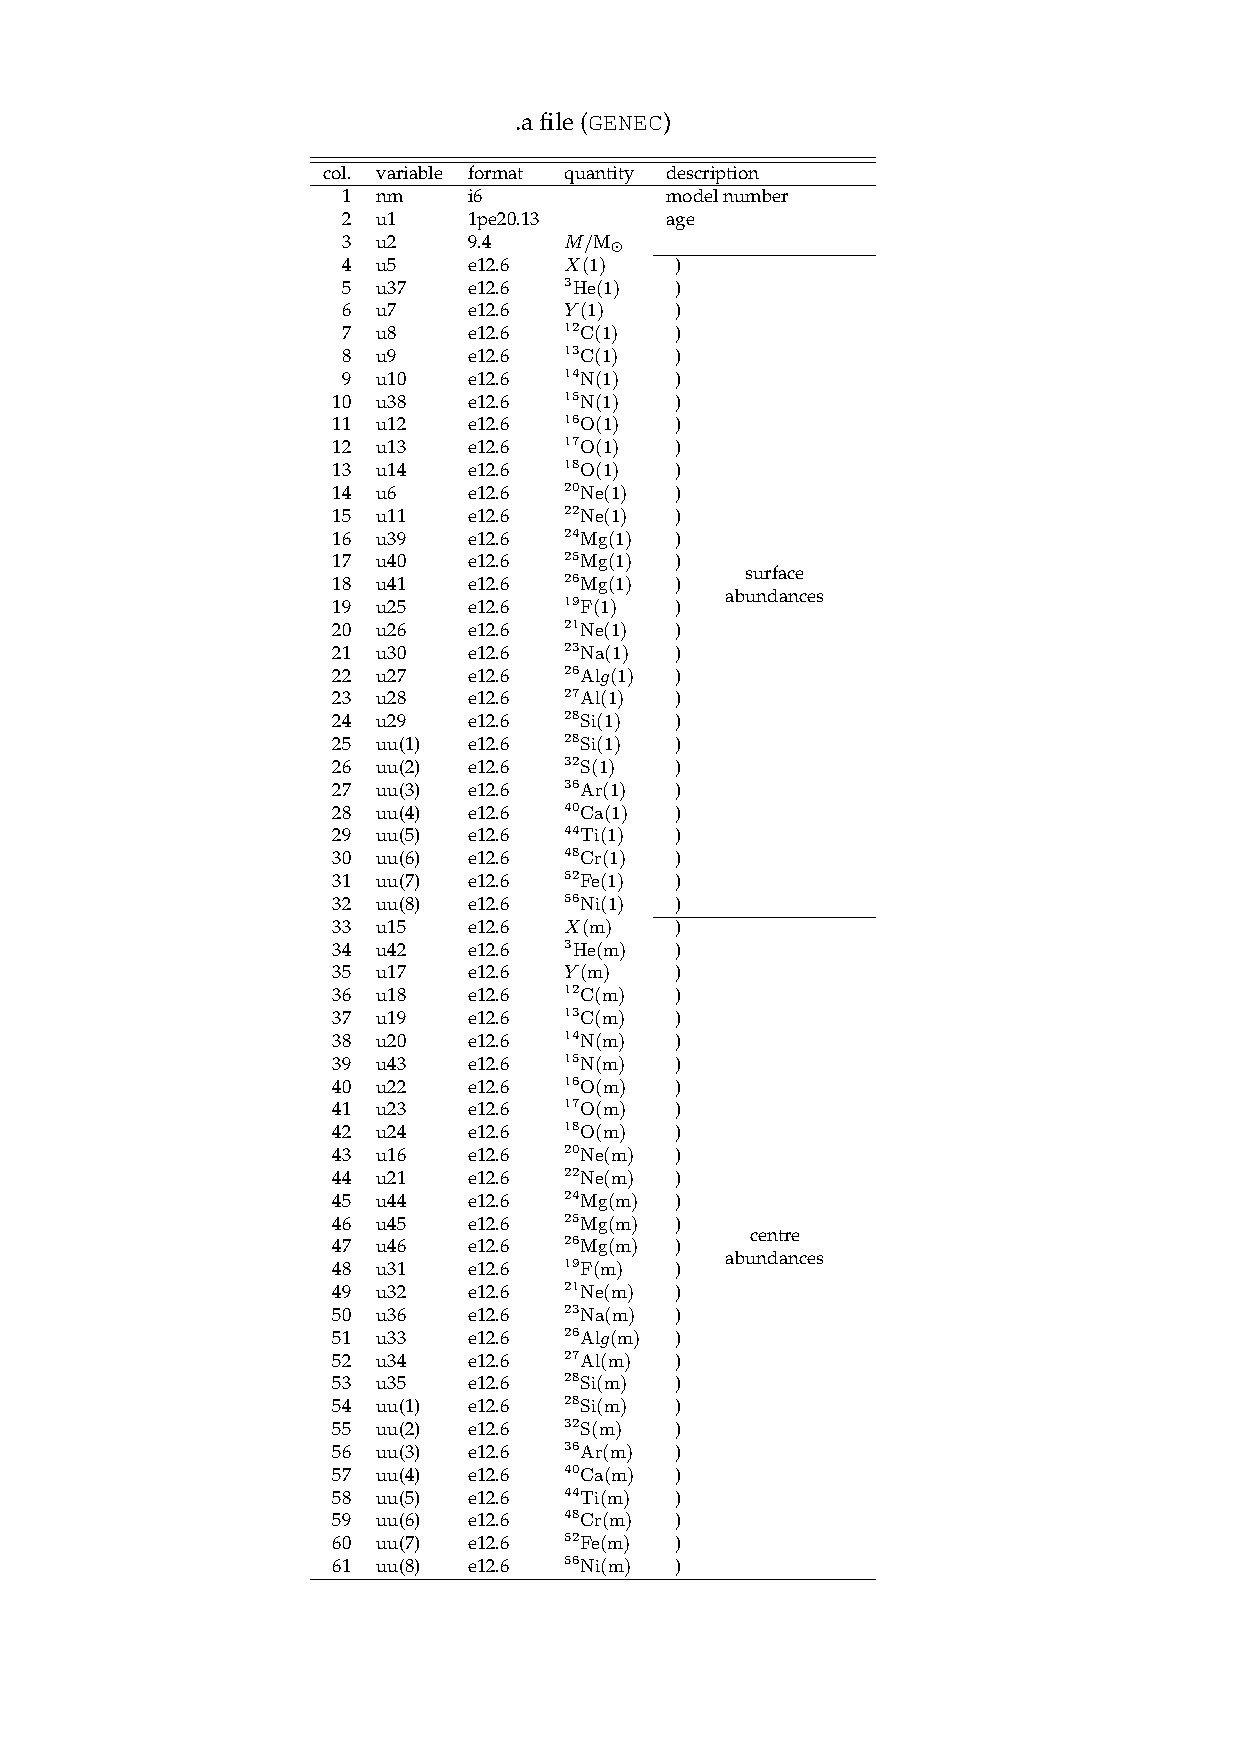
\includepdf[pages=1,scale=0.9,offset=0 -1cm,linkname=afile]{afile_GENEC.pdf}
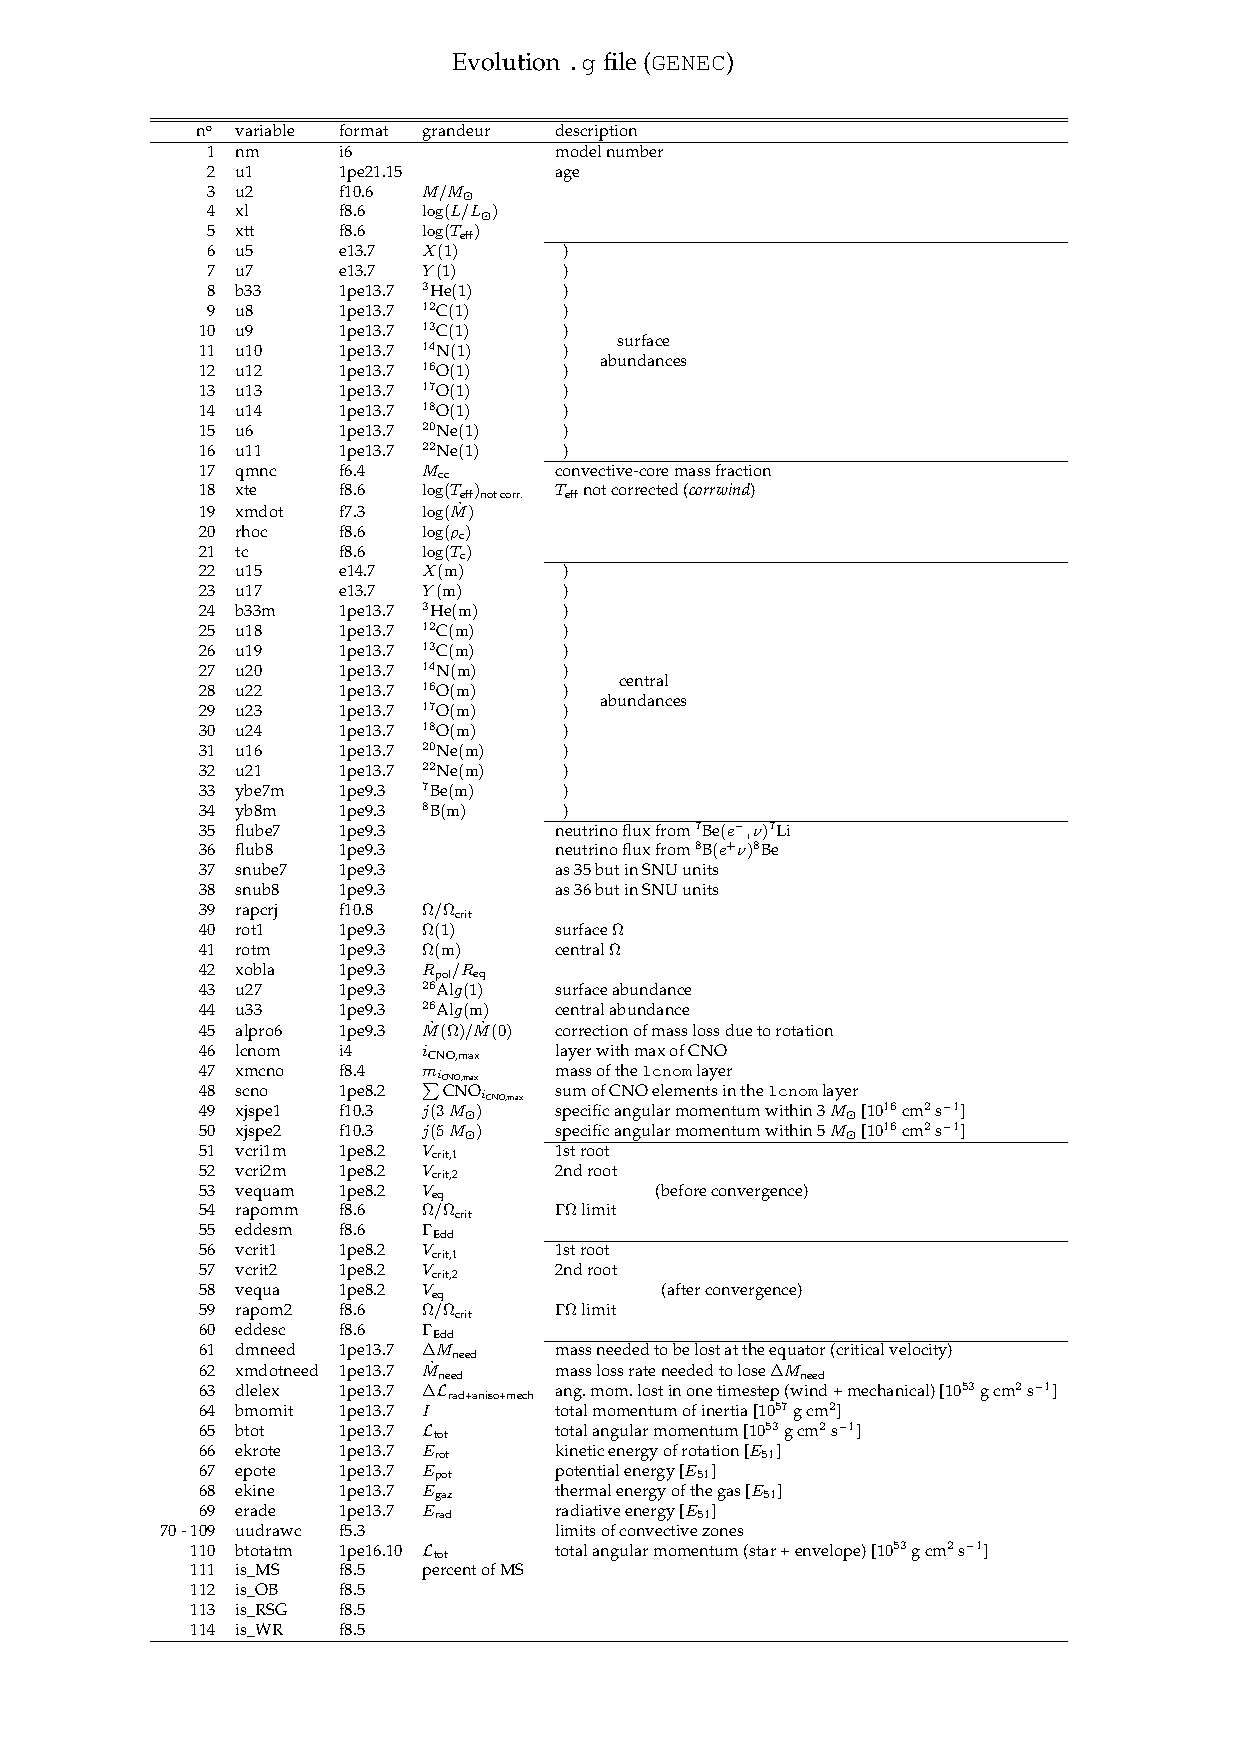
\includepdf[pages=1,scale=0.9,offset=0 -1cm,linkname=gfile]{gfile_GENEC.pdf}
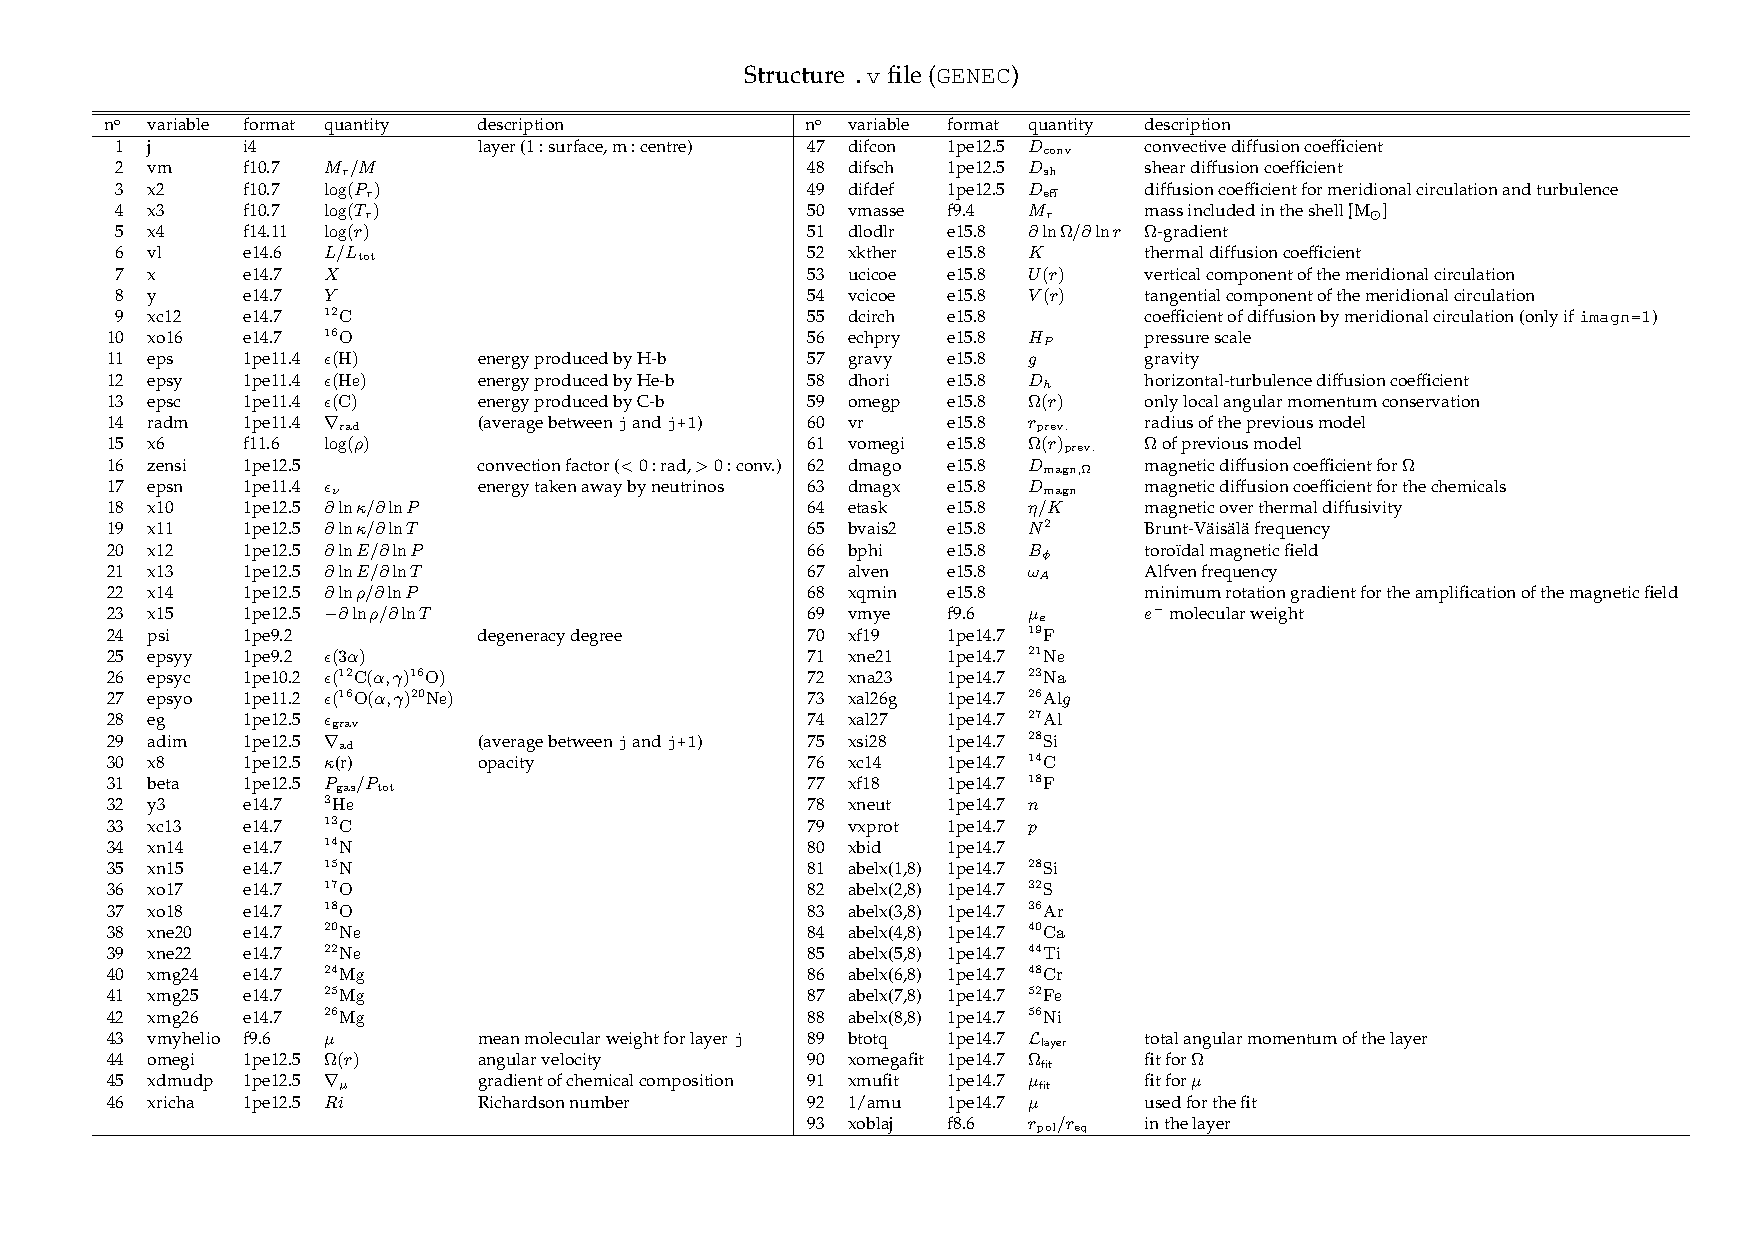
\includepdf[pages=1,offset=0 -1cm,linkname=vfile,angle=90]{vfile_GENEC.pdf}
%********************************************************************************************************
\subsection{Modules\label{sMod}}
Some modules contain only basic variables that are needed in the program and various modules. Others contain a set of variables and subroutines or functions treating the various aspects of the code. The modules are described in the following subsections.

%-----------------------------------------------------------------------------------------------------------------------------------
\subsubsection{Modules containing only variables}
Some variables are used in several modules and need to be declared separately in order to be compiled correctly. 

 \begin{description}[]
 \item[const:] physical and astrophysical constants;
 \item[evol:] dimension of arrays and path to the \texttt{inputs} folder;
 \item[caramodele:] global characteristics of the model (model number, mass, luminosity, age, mass lost, etc ...); 
 \item[diffadvmod:] diffusion, advection; 
 \item[equadiffmod:] coefficients for the resolution of the differential equations used in {\tt henyey} (structure) and {\tt henadv} (advection); 
 \item[rotmod:] rotation variables ($\Omega$, angular momentum, meridional circulation, etc ...); 
 \item[strucmod:] structure variables (pressure, temperature, density, gradients, gravity, etc ...).
 \end{description}

%-----------------------------------------------------------------------------------------------------------------------------------
\subsubsection{Modules containing variables and subroutines}
These modules are a kind of box treating a specific aspect of the physics of the code.

\paragraph{\underline{\texttt{abundmod}}}
This module contains the variables for the chemical abundances, reaction rates, neutrinos, energies. It also contains two subroutines:
 \begin{description}
   \item[abundCheck:] verification that the abundances do not deviate too much from 1;
   \item[maxCNO:] search for the shell with maximal N abundance.
 \end{description}

\paragraph{\underline{\texttt{advection}}}
This module contains the 16 subroutines treating advection:

 \begin{description}
   \item[advect:] centrale routine for the advection computation, calling all other subroutines and modifying eventually the \om\ profile  through advection and / or diffusion.
   \item[badv:] determination of the surface conditions for the henyey methode  resolving advection;
    \item[confi:] determination of the convective zones configuration (rad-conv-rad, conv-rad, conv-rad-conv, fully rad, fully conv, ...);
   \item[coradv:] computation of the difference between advected \om\ and previous \om;
   \item[ebems:] computation of the components $\bar{\epsilon} / \epsilon _\text{m}$ (gravitational and nuclear energy) of meridional circulation;
   \item[echtem:] determination of various components of the meridional circulation;
   \item[gbar:] computation of the mean value for $g$ on an isobar;
   \item[giadv:] computation of the matrix elements corresponding to the 4 equations allowing the resolution of the advective part of  the angular momentum transport equation;
   \item[gtilgm:] computation of $\tilde{g}/\bar{g}$: fluctuation of $g$ on the isobar with respect to the mean $g$ of the shell;
   \item[henadv:]  resolution of the differential equations of advection;
   \item[initia:] initialisation of the meridional circulation according to a simplified expression;
   \item[momcon:] computation of the inertia momentum of the convective zones;
   \item[rechzr:]  search for the radiative and convective zones in the model;
   \item[urs1:] computation of $U_r$, the radial component of the meridional circulation;
   \item[vcirc:] computation of $V_r$, the horizontal component of the meridional circulation;
   \item[ziadv:] as \texttt{giadv}, but for the centre.
\end{description}

\paragraph{\underline{\texttt{bintidemod}}}
This module contains the 2 subroutines treating the tidal effects:

 \begin{description}
   \item[dLtidcalc:] computes the tidal forcing on the surface velocity, according to Zahn (1977);
   \item[orbitalevol:] computes the evolution of the orbital separation due to tides.
 \end{description}

\paragraph{\underline{\texttt{chemicals}}}
This module contains the subroutines treating the modifications of chemical abundances due to nuclear reactions, convection and rotational mixing:

\begin{description}
 \item[chemold:] homogeneisation of the previous abundances on the new convective zones before the call to \texttt{netnew} or \texttt{netwki} ;
 \item[chemeps:] homogeneisation of the nuclear reactions in the convective zones before the call to \texttt{netnew} (in the case of a call to \texttt{netwki}, neutrons and short-lived chemicals are followed, hence no homogeneisation is performed);
 \item[netnew:] computation of the changes in abundances through the nuclear reactions;
 \item[netwki:] idem, but in the case where the NeNa-MgAl network is followed;
 \item[netalu:] called by \texttt{netwki}, computation of the matrix elements for the chemicals and H-b reactions;
 \item[netflu:] idem but for He-b reactions;
 \item[chemie:] homogeneisation of the abundances in the convective zones after \texttt{netnew} or \texttt{netwki};
 \item[mixe:] called by \texttt{chemeps} for the mixing.
 \end{description}

\paragraph{\underline{\texttt{convection}}}
This module contains the routines for the treatment of convection:

\begin{description}
 \item[bordn:] search for the borders of the convective zones;
 \item[over1:] computation of the core size extended by the overshooting;
 \item[unders:] computation of the depth of the external convective zone extended by the undershooting;
 \item[fconva:] convection function for $\ell=\alpha\cdot H_\rho$;
 \item[rechzco:] definition of the configuration type:
   \begin{description}
     \item[iconra=0:] fully convective
     \item[iconra=1:] fully radiative
     \item[iconra=2:] rad----rad
     \item[iconra=3:] conv---conv
     \item[iconra=4:] rad----conv
     \item[iconra=5:] conv---rad;
  \end{description}
 \item[konvek:] counter for the convective zones in the envelope;
 \item[CZdraw:] determination of the limits of the convective zones for writing in the \texttt{.g} file.
\end{description}

\paragraph{\underline{\texttt{diffusion}}}
This module contains all the routines needed to compute the diffusion of chemicals and angular momentum:

\begin{description}
 \item[coedif:] computation of the diffusion coefficients $D_\text{h}$, $D_\text{shear}$, $D_\text{circ}$, $D_\text{conv}$, and $D_\text{magn}$;
 \item[couran:] computation of the Courant conditions for the diffusion of the chemicals;
 \item[courom:] idem for the diffusion of \om;
 \item[diffbr:] resolution of the diffusion equation for the chemicals;
 \item[diffom:] resolution of the diffusion equation for \om.
 \end{description}

\paragraph{\underline{\texttt{energy}}}
This module contains all the routines needed for computing the nuclear reaction rates and the energy generation:

\begin{description}
 \item[energ:] computation of the nuclear reaction rates;
 \item[screen:] computation of the screening factor;
 \item[calcrates:] computation of the nuclear reaction rates and screening factor for the advanced phases;
 \item[interpol:] interpolation in the reaction rates tables;
 \item[netburning:] computation of the abundance modifications due to advanced phases reactions;
 \item[netinit:] initialisation of the advanced phases isotopes network;
 \item[contribreac:] definition of the nuclear reactions considered in the advanced phases;
 \item[readnetZA:] reading of the considered isotopes network;
 \item[readreac:] reading of the considered nuclear reactions;
 \item[inversmat:] inversion of the matrix for the abundance changes due to advanced phases reactions;
 \item[nucal:] computation of the solar neutrino flux;
 \item[nuint:] computation of the integral for the solar neutrino flux;
 \item[enint:] computation of the internal energies of the model:
   \begin{itemize}
     \item gravitational potential energy;
     \item rotational energy;
     \item kinetic energy of the gas;
     \item radiative energy.
   \end{itemize}
 \end{description}

\paragraph{\underline{\texttt{envelope}}}
This module treats the envelope and the atmosphere layers:

\begin{description}
 \item[dreckf:] computation of the three $\alpha,\beta,\gamma$ of the triangle;
 \item[dreck:] computation of the triangle;
 \item[ggw:] computation of $P$, $T$, and $r$ of the envelope and atmosphere;
 \item[atmos:] integration of the atmosphere;
 \item[anfitg:] determination of the conditions in the three first layers of the envelope;
 \item[diff3:] integration  of the envelope;
 \item[rsgl:] computation of the right-hand side of the structure equations in the envelope;
 \item[rsgl1:] idem, but in the case of massive stars, with the turbulent pressure taken into account;
 \item[print1:] printing of the structure of the envelope.
 \end{description}

\paragraph{\underline{\texttt{EOS}}}
This module computes the EOS of the model:

\begin{description}
 \item[degen:] computation of the EOS in the degenerate case;
 \item[Compute\_sepp:] computation of the variables needed for the EOS (called by \texttt{dichte});
 \item[dichte:] comutations of the EOS.
 \end{description}

\paragraph{\underline{\texttt{geomod}}}
This module contains the small routines used to interpolate in the table \texttt{ftfp.dat}:

\begin{description}
 \item[initgeo:] reading of the table \texttt{ftfp.dat};
 \item[geocalc:] interpolation in the table (general application);
 \item[geomat:] from $S_\psi$ determination of $r_\psi$, $S_\text{isobare}/(4\,\pi\,r_\psi^2)$, $f_T$, $g(x_\psi)/\left<g\right>$, and $\left<g^{-1}\right>$ ;
 \item[geomeang:] from $r_\psi$ determination of $\left|\left|g(x_\psi)\right|\right|\cdot\left(\left<g^{-1}\right>/g(x_\psi)\right)$ ;
 \item[geomEdd:] determination of the maximal $\Gamma_\text{Edd}$ given the value for $\Omega/\Omega_\text{crit}$ ;
 \item[geom:] from $r_\psi$ determination of $f_P$ and $f_T/f_P$
 \end{description}

\paragraph{\underline{\texttt{henyey}}}
This module contains the routines used for the resolution of the structure equations with the Henyey method:

\begin{description}
 \item[printheynyey:] writing of the \texttt{.v} file containing the description of the internal structure;
 \item[Calcvmyhelio:] computation of the solar neutrino emission and of $\mu$ ;
 \item[gisu:] computation of the elements of the equations $G_{1,2,3,4}$ with the possibility to apply the shift of the point in the shell where the values are computed (\href{https://ui.adsabs.harvard.edu/abs/1970ApJ...159..619S}{Sugimoto 1970}, used for the advanced phases);
 \item[gi:] idem in the normal case;
 \item[zi:] computation of the elements of the equations $Z_{1,2,3,4}$;
 \item[henyey:] resolution of the structure equations with the Henyey method.
 \end{description}

\paragraph{\underline{\texttt{inputparam}}}
This module contains all the variables of the parameters card, as well as the routines that control the changes brought to these parameters:

\begin{description}
  \item[Write\_param:] writing of the input parameters if they are not set to their default value;
 \item[Write\_namelist:] writing of the parameters card;
 \item[Read\_namelist:] reading of the parameters card;
\item[FITM\_Change:] computation of the changes in \texttt{FITM} during the crossing of the HR diagram;
 \item[IMLOSS\_Change:] change of the radiative mass-loss prescription if the model enters a new phase;
 \item[INPUTS\_Change:] change of the input parameters depending on the evolutive stage and the current situation of the model;
 \item[Ask\_changes:] change of the input parameters when creating the initial file.
\end{description}

\paragraph{\underline{\texttt{interpolation}}}
This module contains the small routines used for linear or quadratic interpolations, and splines:

\begin{description}
 \item[indic,fipoi,fipoi1,fipoi2,quint,qua,quad,quad\_gg,flin,spline,splint,getd.]
 \end{description}

\paragraph{\underline{\texttt{ionisation}}}
This module contains the routines computing the ionisation:

\begin{description}
 \item[ionpart:] computation of partial ionisation for H, He, C, O, Ne, Mg;
 \item[saha:] resolution of Saha equation.
 \end{description}

\paragraph{\underline{\texttt{LayersShift}}}
This module contains the routines controlling the layers adjustments and the mesh refinement:

\begin{description}
 \item[FITMshift:] readjustment of the layers after a change in \texttt{FITM};
 \item[MdotShift:] readjustment of the layers after mass loss;
 \item[schrit:] addition or suppression of layers according to the variations of given variables from one layer to the next ($M$, $L$, $r$, $P$, $\Omega$, $X_\text{H}$, $X_\text{He}$, $X_{^{12}\text{C}}$, $X_{^{16}\text{O}}$, $X_{^{20}\text{Ne}}$ ;
 \item[interx:] interpolation sub-routine used to readjust the values of the variables in the layers that have been modified.
 \end{description}

\paragraph{\underline{\texttt{magmod}}}
This module contains the variables of the magnetic field, and the routine that computes them:

\begin{description}
 \item[Mag\_diff:] computation of the variables of the magnetic field, and of the magnetic diffusion coefficients $D_\text{mag,X}$ et $D_{\text{mag,}\Omega}$ (not used anymore);
 \item[Mag\_dif\_general:] computation of the magnetic instabilities according to three prescriptions (selected by the \texttt{n\_mag} parameter):
 \begin{enumerate}[labelindent=.5cm,font=\ttfamily \bfseries,label=\arabic*:]
   \item classical Tayler-Spruit implementation (default value);
   \item modified TS implementation;
   \item Fuller+ 2019 implementation.
 \end{enumerate}
\end{description}

\paragraph{\underline{\texttt{nablas}}}
This module contains the routines computing the nablas.

\begin{description}
 \item[nabla:] computation of $\nabla_\text{rad}$ and $\nabla_\text{ad}$, with their derivatives;
 \item[nabgam:] computation of $\nabla$ in the whole star according to Eq. (6.39) in Maeder (1997);
 \item[grapmui:] computation of $\nabla_\mu$.
 \end{description}

\paragraph{\underline{\texttt{nagmod}}}
This module contains the {\tt NAG} routines used by the program:

\begin{description}
 \item[c02agf:] computation of the roots of a real polynomial equation of {\tt n} degrees;
 \item[e02acf:] computation of a minimax polynomial fit on a set of points, through Chebyshev polynomials;
 \item[a02aaf,a02abf,a02acf,c02agt,c02agu,c02agv,c02agw,c02agx,c02agy,c02agz,f06blf:] routines called by the two main ones.
 \end{description}

\paragraph{\underline{\texttt{omega}}}
This module contains the routines treating \om:

\begin{description}
 \item[VcritCalc:] computation of $V_\text{crit,1}$, $V_\text{crit,2}$, $V_\text{eq}/V_\text{crit}$, and $\Omega/\Omega_\text{crit}$;
 \item[dlonew:] computation of $\text{d}\ln \Omega/\text{d}\ln r$;
 \item[omenew:] approximate computation of $\Omega(r)$ on the basis of the angular momentum of the previous iteration applied on the new structure;
 \item[omescale:] computation of the correction to apply to the rotation profile to ensure the conservation of angular momentum after mass loss, and repartition of the correction on a given number of layer under the surface;
 \item[OmegaReset:] verification that the correction of the angular momentum did not cause $\Omega<0$ in some layers. if yes, the zones are set to 0 and the correction is recomputed;
 \item[omconv:] computation of $\Omega(r)$ in convective zones;
 \item[momevo:] computation of the total angular momentum;
 \item[mominertenv:] computation of the inertia momentum of the envelope;
 \item[vomcon:] computation of the initial $\Omega(r)$, homogenised in the convective zones, before applying local conservation, diffusion, and advection;
 \item[momspe:] computation of the specific angular momentum;
 \item[omenex:] approximatecomputation of $\Omega(r)$ for the next model;
 \item[om2old:] computation of the inertia momentum (used by \texttt{omenex});
 \item[omesta:] computation of $\Omega(r)$ in case only the local conservation of angular momentum is taken into account (\verb?ISTATI=1, IDIFF=0?).
 \end{description}

\paragraph{\underline{\texttt{opacity}}}
This module contains the routines computing the opacity.

\begin{description}
 \item[opacgn93:] determination of the table(s) to be used;
 \item[opac,t6interp,readco,opaltab,fity,fitx,interp,smooth:] sub-routines of the opacity computation recursively called by opacgn93;
 \item[kappa\_out:] extrapolation of the opacity if the conditions on $T$ and $\rho$ are out of the tables;
 \item[condTest:] test if conductive opacity has to be computed;
 \item[cond:] computation of the conductive opacity;
 \item[kappa:] front door routine for the computation of the opacities. Calls \texttt{opacgn93} or \texttt{kappa\_out} depending if the conditions are inside the opacity tables or outside.
 \end{description}

\paragraph{\underline{\texttt{PGPlotModule}}}
This module contains all the routines linked to the direct visualisation through \texttt{pgplot}. Note that for systems where \texttt{pgplot} could not be installed, an alternative version \texttt{PGPlotModuleNull} without the \texttt{pgplot} commands is present in the source directory and becomes effective if the \texttt{PGPLOT} parameter in the makefile is set to \texttt{FALSE}.

\begin{description}
  \item[InitPGplot:] initialisation of the module and X windows;
  \item[SavePlotData:] saving all the data needed to plot the evolution window, stored in \texttt{.PlotData\_starName}. Uses \texttt{Estimate\_Lifetime}, and calls \texttt{FindCZ}, \texttt{Find\_Max\_Energy}, and the plotting routines \texttt{PlotEvol} and \texttt|{PlotStruc};
  \item[FindCZ:] search of the convective zones, needed for the Kippenhahn diagram of the evolution window. Calls \texttt{Mass\_Vector};
  \item[Mass\_Vector:] definition of the mass mesh for the Kippenhahn diagram ($y$ axis);
  \item[Estimate\_Lifetime:] estimation of the MS lifetime, based on a fit on Ekstr\"om+ 2012, used to set the time tolerance (max timestep between two plotted models if no other variable changed enough for triggering the plotting);
  \item[Find\_Max\_Energy:] saving the location of the maximal energy generation of the various burnings for the Kippenhahn diagram;
  \item[PlotEvol:] plot of the evolution window;
  \item[PlotStruc:] plot of the structure window;
  \item[EndPGplot:] closing of file and end of module.
\end{description}

\paragraph{\underline{\texttt{PrintAll}}}
This module contains the routines storing and printing the complete model (interior, envelope, and atmosphere):

\begin{description}
 \item[StoreStructure\_int,StoreStructure\_env,StoreStructure\_atm:] storage of the variables of the layers;
 \item[PrintCompleteStructure:] printing of the complete structure.
\end{description}

\paragraph{\underline{\texttt{SmallFunc}}}
This module contains all sorts of small routines and general functions:

\begin{description}
 \item[girl:] inversion of a matrix;
 \item[CheckProfile:] verification that a curve is smooth, and elimination of the jump if there is one;
 \item[SmoothProfile:] smoothing of a curve by the \textit{locally weighted scatterplot smoothing} technique;
 \item[tridiago:] resolution of the diffusion equation;
 \item[weighed\_smoothing:] smoothing of a variable over a defined number of shells;
 \item[threshold\_smoothing:] same as above but only if the variable is larger than the threshold;
 \item[primus,drimus:] function $f=\frac{a}{T_9^{e1}}\,\cdot\,\exp(-\frac{b}{T_9^{e2}})$ and the derivative, used for the analytical computation of reaction rates in \texttt{energ};
 \item[secun,dsecun:] idem, function $f=\frac{a}{T_9^{e1}}\,\cdot\,\exp\left(-\frac{b}{T_9^{e2}}-\left(\frac{T_9}{c}\right)^{e3}\right)$ and derivative;
 \item[tertiu,dterti:] idem, function $f=a+b\,\cdot\,T_9^{e1}+c\,\cdot\,T_9^{e2}+d\,\cdot\,T_9^{e3}+e\,\cdot\,T_9^{e4}+f\,\cdot\,T_9^{e5}$ and derivative;
 \item[expf10:] $\ln$ to $\log_{10}$ function: $f=\exp\left(\frac{x}{\log_{10}(e)}\right)$;
 \item[exphi:] function $f=1-\exp(x)$ with limited series expansion if $|x| \leq 0.03$: $f=-\left(\left(\frac{x}{3} + 1 \right)\cdot\frac{x}{2} + 1\right)\cdot x$;
 \item[pos:] search for the position of a value in a monotonic table (increasing or decreasing);
 \item[ValInterp:] interpolation function $f=\frac{x_1\cdot(y_2-y_3)+x_2\cdot(y3-y1)}{y_2-y_1}$;
 \item[OmInterp:] interpolation function $f=\frac{x_1\cdot(y_2-y_3)\cdot z_1+x_2\cdot(y_3-y_1)\cdot z_2}{(y_2-y_1)\cdot z_3}$.
 \end{description}

\paragraph{\underline{\texttt{timestep}}}
This module contains the routines controlling the time steps:

\begin{description}
 \item[zeit:] computation of the next time step;
 \item[TimestepControle:] adaptation of \texttt{xcn} depending on the situation of the model.
 \end{description}

\paragraph{\underline{\texttt{winds}}}
This module contains the routines linked to mass loss:

\begin{description}
 \item[xloss:] computation of the radiatively-driven mass loss;
 \item[xldote:] Computation of the loss of angular momentum;
 \item[dLmagcalc:] computation of the loss of angular momentum due to magnetic braking;
 \item[dLmagLM:] computation of the loss of angular momentum due to magnetic braking in low-mass stars (Kawaler 1988);
 \item[aniso:] computation of the wind anisotropy;
 \item[corrwind:] correction of \teff\ for the wind thickness;
 \item[Compute\_MagCorrection:] computes the reduction of the mass-loss rates due to magnetic quenchiing (Petit+ 2016)
 \end{description}

\paragraph{\underline{\texttt{WriteSaveClose}}}
This module contains the routines that start and end the computation of a series of time steps:

\begin{description}
 \item[write4:] storing of the initial model at the beginning of a model computation;
 \item[read4:] reading of the model stored in \texttt{write4};
 \item[SequenceClosing:] closing of a series of models;
 \item[OpenAll:] opening of the input/output files;
 \item[CloseAll:] closing of the input/output files.
 \end{description}

%\includepdf[linkname=OriginTools]{OriginTools_Manual.pdf}
%\includepdf[linkname=svn]{svn_origin2010.pdf}
%********************************************************************************************************
\end{document}
% \includegraphics[height=6cm]{figname.pdf}
